\documentclass{article}
\usepackage{amsmath}
\usepackage{graphicx}
\usepackage{siunitx}  % For better unit handling
\usepackage{enumitem} % For better list handling

\begin{document}

\section*{Part I: Solve any six questions}

\subsection*{1. Differentiate between accuracy, precision and resolution}
Accuracy refers to the closeness of a measured value to a standard or known value. Precision indicates the closeness of two or more measurements to each other. Resolution is the smallest increment that a measurement device can detect and display.

\subsection*{2.}
\subsubsection*{(a) Five important components of a lathe machine}
\begin{enumerate}[label=\arabic*.]
    \item Bed
    \item Headstock
    \item Tailstock
    \item Carriage
    \item Feed mechanism
\end{enumerate}

\subsubsection*{(b) Stepper motor vs Servomotor}
\begin{itemize}
    \item \textbf{Stepper Motor:} Moves in discrete steps, no feedback loop, suitable for open-loop systems.
    \item \textbf{Servomotor:} Continuous motion with feedback loop, suitable for closed-loop systems.
\end{itemize}

\subsubsection*{(c) Ten important parameters of the specification of a lathe machine}
\begin{enumerate}[label=\arabic*.]
    \item Swing over bed
    \item Distance between centers
    \item Spindle bore
    \item Spindle speed range
    \item Feed rates
    \item Chuck size
    \item Motor power
    \item Tailstock quill travel
    \item Bed width
    \item Weight of the machine
\end{enumerate}

\subsection*{3. Determination of shear strength of work material}
Given: 
\begin{itemize}
    \item Cutting force, $F_c = \SI{1470}{N}$
    \item Thrust force, $F_t = \SI{1589}{N}$
    \item Rake angle, $\alpha = \SI{5}{\degree}$
    \item Chip thickness ratio, $r = 0.38$
\end{itemize}

From Merchant's equation:
\begin{equation}
    \phi = \tan^{-1}\left(\frac{r \cos \alpha}{1 - r \sin \alpha}\right)
\end{equation}

Substituting the given values to find $\phi$, then use:
\begin{equation}
    F_s = F_c \cos \phi - F_t \sin \phi
\end{equation}

\subsection*{4. Power drawn by the lathe in turning operation}
Given:
\begin{itemize}
    \item Cutting speed, $V = \SI{150}{m/min}$
    \item Feed, $f = \SI{0.25}{mm/rev}$
    \item Depth of cut, $d = \SI{7.5}{mm}$
    \item Mechanical efficiency, $\eta = \SI{90}{\percent}$
    \item Specific energy, $u = \SI{2.8}{N.m/mm^3}$
\end{itemize}

Power required:
\begin{equation}
    P = \frac{u \times V \times f \times d}{\eta}
\end{equation}

\subsection*{5. Cutting speed for specified machining time}
Given:
\begin{itemize}
    \item Length, $L = \SI{375}{mm}$
    \item Diameter, $D = \SI{150}{mm}$
    \item Feed, $f = \SI{0.30}{mm/rev}$
    \item Depth of cut, $d = \SI{4.0}{mm}$
    \item Machining time, $T = \SI{5.0}{min}$
\end{itemize}

Calculate cutting speed $V$:
\begin{equation}
    V = \frac{L}{T \times f}
\end{equation}

\subsection*{6. Cutting time for drilling operation}
Given:
\begin{itemize}
    \item Drill diameter, $D = \SI{12.7}{mm}$
    \item Depth, $L = \SI{60}{mm }$
    \item Feed, $f = \SI{0.25}{mm/rev}$
    \item Spindle speed, $N = \SI{500}{rpm}$
\end{itemize}

Calculate cutting time $T$:
\begin{equation}
    T = \frac{L}{f \times N}
\end{equation}

 If you have the image files, uncomment the following lines
 \begin{center}
     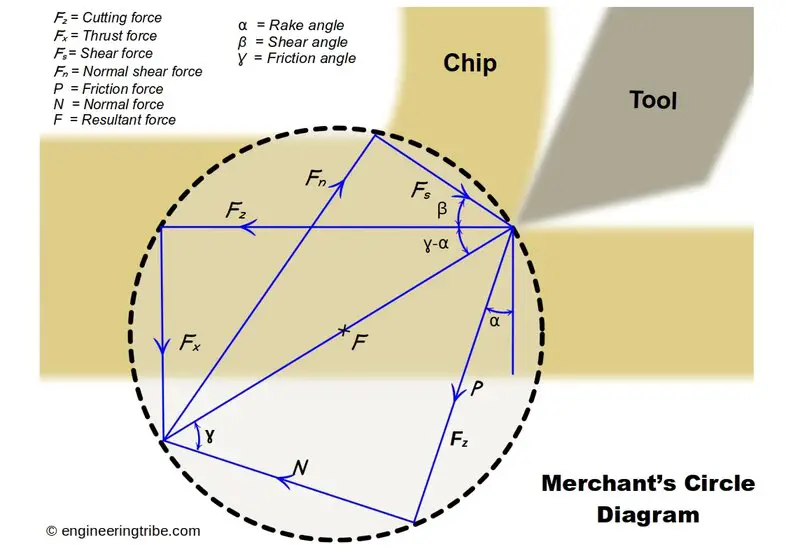
\includegraphics[width=\textwidth]{merchant_circle.png}
 \end{center}

 \begin{center}
     \includegraphics[width=\textwidth]{tool_nomenclature.png}
 \end{center}

\end{document}